\documentclass[11pt]{report}
% packages
% Fran Burstall's Bath thesis package
\usepackage{baththesis}
\usepackage{amssymb} %for Blackboard bold etc \usepackage{graphicx} %for including eps graphics % front matter
\usepackage[pdftex]{graphicx}
\usepackage{url}

\title{ Illustrating how hydraulic machinery works } \author{Garoe Dorta-Perez}
%\degree{Doctor of Philosophy}
\degree{ Master of Science }
\department{Department of Computer Sciences} \degreemonthyear{January 2015}
\norestrictions

\begin{document}
\maketitle
\begin{abstract}
In this research proposal we present a method for automatic depiction of how it works illustrations of hydraulic machinery. \end{abstract}


\chapter{Introduction}
\label{ch:intro}
In the field of hydraulics, simulations can be used to illustrate how hydraulic machinery works.
A common hydraulic equipment has 
some type of liquid fluid that becomes pressurised when a force is applied to it and then
that force is transmitted to the other end of the fluid. Understanding how the pressured is
directed and how it interacts with other parts in the machinery is essential in order
to grasp how the whole system works. Therefore in order to illustrate the general 
process the user needs to know the spatial configuration of all the parts in the
system and the chain of motions that takes place within the gears and the liquid fluids
as well.

This research proposal aims to introduce an automatic method for generating
illustrations on how things work on hydraulic machinery. 

In summary, the main contributions would be:
\begin{itemize}
\item An application for creating how things works illustration for hydraulic machinery 3D models.
\item A method for detecting motion and interaction of fluid inside 3D model parts.
\item Algorithms to automatically generate illustrations with motion arrows and frame sequences
\end{itemize}

Don't forget how to cite \cite{Burstall} and reference, like Chapter \ref{ch:intro}

\section{The Problem}
\label{sec:problem}
\begin{figure}[htb]
  \centering
    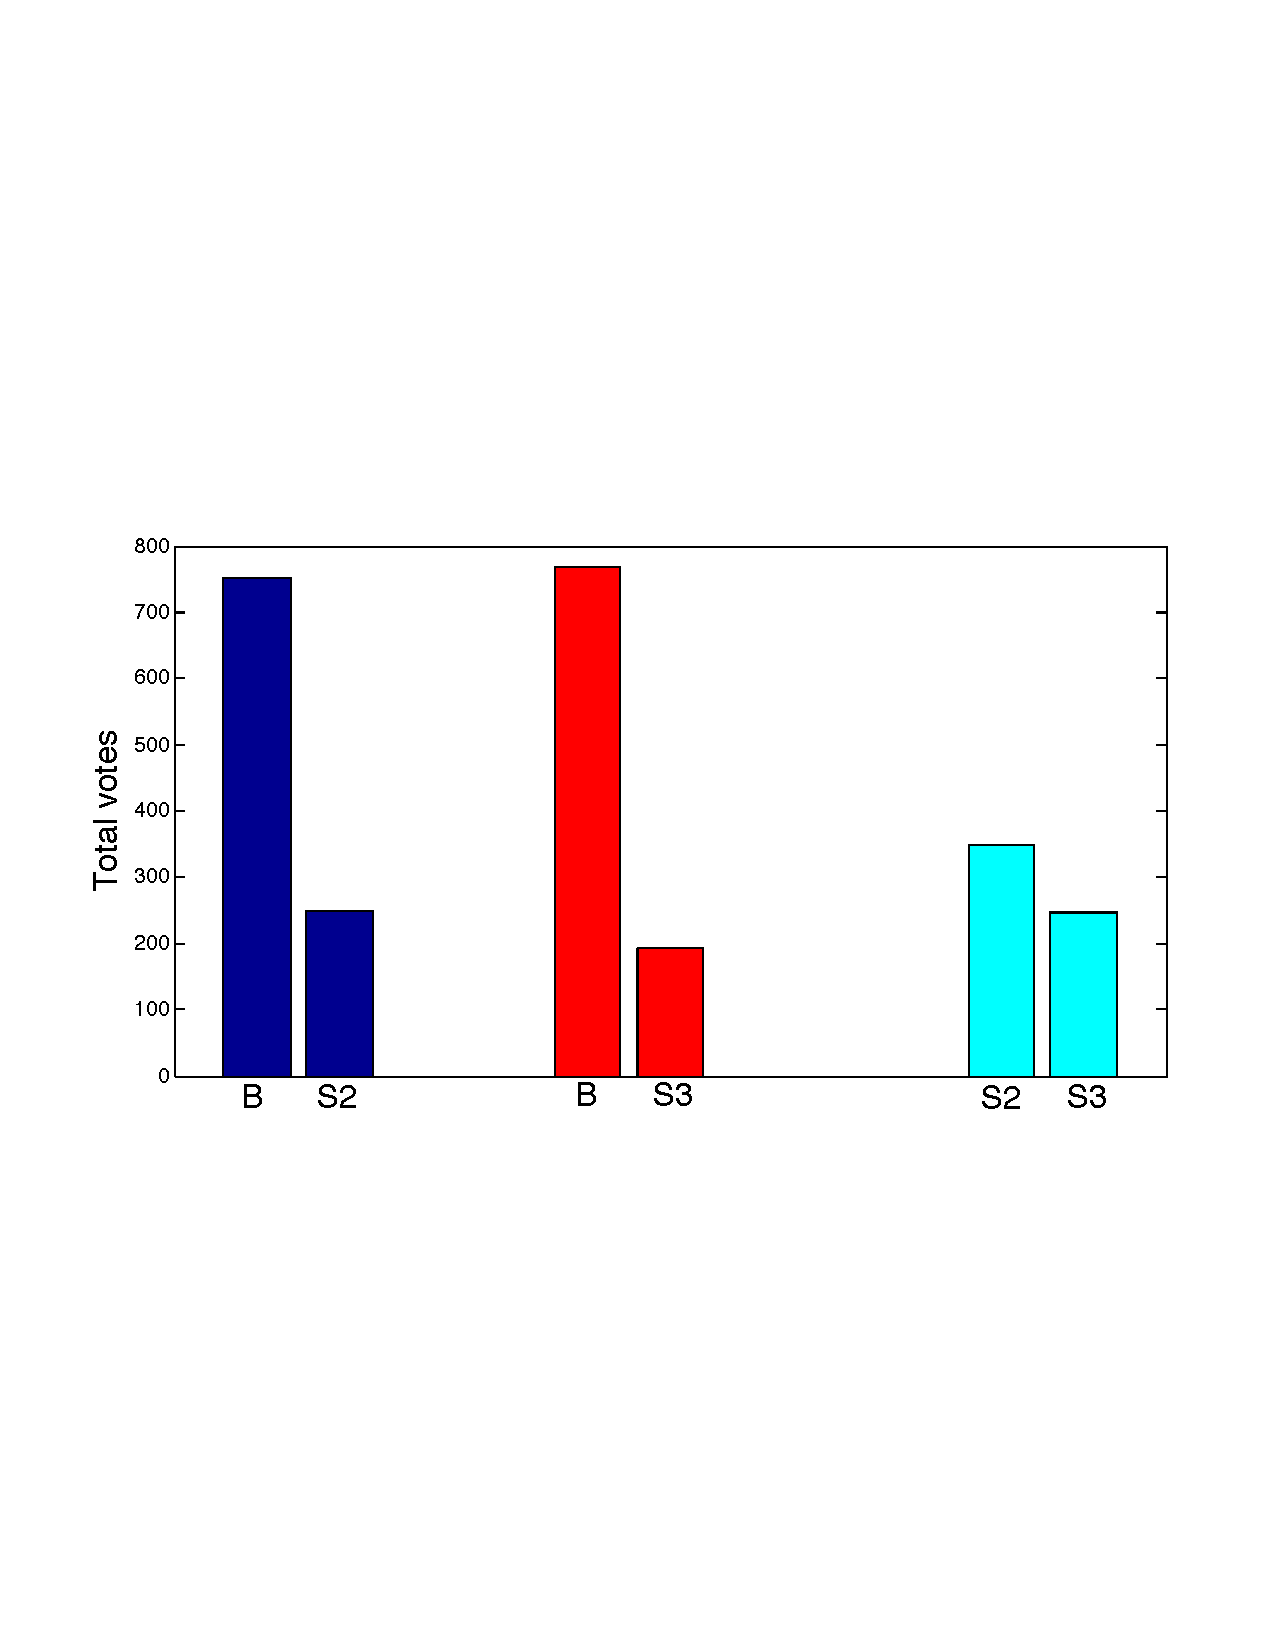
\includegraphics[width=.8\linewidth]{images/allComparison.pdf}
  \caption{\label{fig:all}
           An unrelated bar chart.}
\end{figure}

We begin by divulging the third secret of the Universe, namely that if I told you I would have to kill you.
This is not really illustrated by the irrelevant Figure~\ref{fig:all}
Grasping this fact enables us to move quickly into the next chapter.

\begin{figure}[htb]
  \centering
    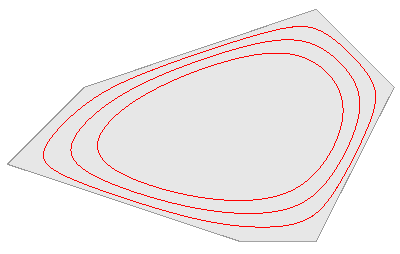
\includegraphics[width=.8\linewidth]{images/unweightedlog6.png}
  \caption{\label{fig:unweightedlog6}
           Three example curves.}
\end{figure}

\section{Previous Work}

This proposal is based on the following three main areas of previous work.

\subsection{Explanatory illustration}

This method effectively conveys the explanatory information to the user. Researchers
have have developed several automatic techniques for a range of problems. \cite{Mitra2010}
There are no earlier references to the problem outlined in \ref{sec:problem} and earlier work on eight dimensional harmonic maps in general was not done by notables such as Newton in \cite{principia}.

\subsection{Fluid simulation}
No work was done whatsoever in the middle years, and was not mentioned at all in the theory of relativity \cite{einstein}.

\subsection{Flow visualization}
Many authors have commented on the irrelevance of the Wyvill method \cite{Wyvill:1999p149}, which
is not at all illustrated by Figure~\ref{fig:unweightedlog6}.

\subsection{Shape analysis}

\chapter{Data Structures Used in this research}
\section{The 4D-Stack - A Revolutionary Data Structure}
The 4D-Stack turned out to be a complete disaster as traversal time approached $O(n^9).$
It is best illustrated by the following equation: $F(x) = \prod_{0\leq i<k}d_i(x)$
but the following may not be true:

\[
-f(x) = - \log \prod_{0\leq i<k}d_i(x) = - \sum_{0\leq i<k} \log d_i(x)
\]


\section{More Irrelevant Stuff}
If you want to put numbers on equations use this form:
\begin{equation}
\label{integralrep}
f(x)=\int_0^L h( \langle x-p(t),n(t) \rangle ) dt\,.
\end{equation}



\chapter{Results}
\begin{table}[tbp]
\begin{tabular}{||l|l|l|p{1.5in}|p{1.2in}||}
\hline
\hline
Name & Dates & Degree & Title & Present Position \\
\hline
Rudolphe Neyrouge & 1953  - & PhD &  Non-linear Fictional Analysis &  co-tutelle with NPole University, Arctic \\
Rip van Winkle & 1754 -  & PhD & Modelling 4D Harmonic Maps & University of Old People \\

\hline
{\bf Graduated} &&&& \\
\hline
Johnny Depp & 1967 - 2009 & MSc & How to Act an MSc & Actor \\
Valentina Lsitsa & 1992 - 2013 & MSc & Hitting the right notes &  Pianist  \\
Johann S. Bach & 1567 - 1953 & MSc & Interactive Piano  & Composer \\\hline
\hline
\end{tabular}
\caption{\label{stud-table} Graduate Students, last seven years.}
\end{table}

Due to a time quake during the research, the results were catapulted into the future.  They will appear in about 20 years.
In the meantime to demonstrate the use of tables, please see table~\ref{stud-table} for a list of students who took more than 30 years to graduate.

\chapter{Conclusions and Future Work}
No conclusions can be drawn until the results appear and no future work is recommended.

\bibliographystyle{eg-alpha-doi}

\bibliography{baththesis}


\end{document}
